\documentclass{beamer} 
%\documentclass[handout]{beamer} 

% Michael Maier, 2014.
% CC-BY-SA 3.0 at

\usepackage[utf8]{inputenc}
\usepackage[ngerman]{babel}

\title{OpenStreetMap - Die freie Weltkarte} 
\author{Michael Maier \textless Michael.Maier@student.tugraz.at\textgreater} 
\date{26. November 2014} 

\usetheme{Antibes}

\hypersetup{colorlinks=true,urlcolor=blue,linkcolor=white}

%\usebackgroundtemplatei{
%
\includegraphics[width=\paperwidth,
%height=0.8\paperheight]{mag_map.png}
%}

\begin{document}

%\maketitle

\begin{frame} 


\begin{figure}
  \centering
  
\includegraphics[width=.5\textwidth]{mag_map.pdf}
\end{figure}

\begin{center}
\Huge{OpenStreetMap\\}
\end{center}

\begin{center}
\Large{\emph{Die freie Weltkarte}}
\end{center}

\end{frame}


% Zielgruppe
% * Profs und Doktoranden

% tolle Bilder herzeigen!
% * irgendein Zoo
% * 3D
% * Tolle Kartenstile:
%     * OSM-Fr?
%     * stamen watercolor
%     * pistemap
%     * bicycle map
%     * OpenSeaMap
%
% Dokumentation (nenne es doku und nicht Wiki → verwirrent) -OK
% wenn wo doku fehlt, selber mitschreiben?

% Vorteile
% * aktuell!
%
% * Datenversionierung! -OK
% * Language-Independent -OK
%   show http://toolserver.org/~osm/locale/ru.html
% * jetzt in 3D!

% * kurze OSM-Vorstellung, Geschichtliches, Motivation -OK
% * Technogie, Datenmodell, Lizenz -OK
% * OSM Nutzen: Rohdaten, Web-Dienste, Apps


\section{Einleitung}

\begin{frame}{Vorstellung}

  \begin{itemize}
    \item Michael Maier \textless \href{mailto:Michael.Maier@student.tugraz.at}{Michael.Maier@student.tugraz.at}\textgreater
    \item Student an der TU Graz (Telematik)
    \item Verwende Open Source (Debian GNU/Linux) seit 2004
    \begin{itemize}
        \item Organisiere Grazer Linuxtage seit 2011 mit
    \end{itemize}

\vspace{0.15cm}
    \item OpenStreetMap als Hobby seit Juli 2010
    \begin{itemize}
        \item Leite den Grazer OSM-Stammtisch seit Mai 2011
        \item Vorträge und Workshops zum Thema OSM seit 2011
        \item Freiberuflich OSM-Aufträge und Consulting
    \end{itemize}
\vspace{0.3cm}
    \item Open Government Data Meetup Graz seit Beginn
    \begin{itemize}
        \item Betreibe \href{http://opendatagraz.at}{www.opendatagraz.at}
        \item Versioniere OGD auf github
    \end{itemize}
  \end{itemize}
\end{frame}



% Folien zu
% * kurze OSM-Vorstellung, Geschichtliches, Motivation
%  1. OSM-Vorstellung
  % was ist es
  % wer steckt dahinter?
% Geschichtliches
  % Gegründet ... steve
  % user-wachstum
% Motivation
  % gegründet, weil es keine freien Geodaten gab
  % Wunschtraum: eine DB weltweit

\section{OpenStreetMap}

\begin{frame}{Was ist OpenStreetMap}

\begin{itemize}
  \item OpenStreetMap (OSM) ist eine freie Weltkarte nach dem Wiki-Prinzip "`Wikipedia der Karten"'
    \begin{itemize}
      \item \emph{Eigentlich eine Geo-Datenbank}
    \end{itemize}
\pause
  \item Entsteht aus der Arbeit von \textgreater 1,8\,M Hobbykartografen "`\emph{Mapper}"'

\end{itemize}


 \begin{center}
 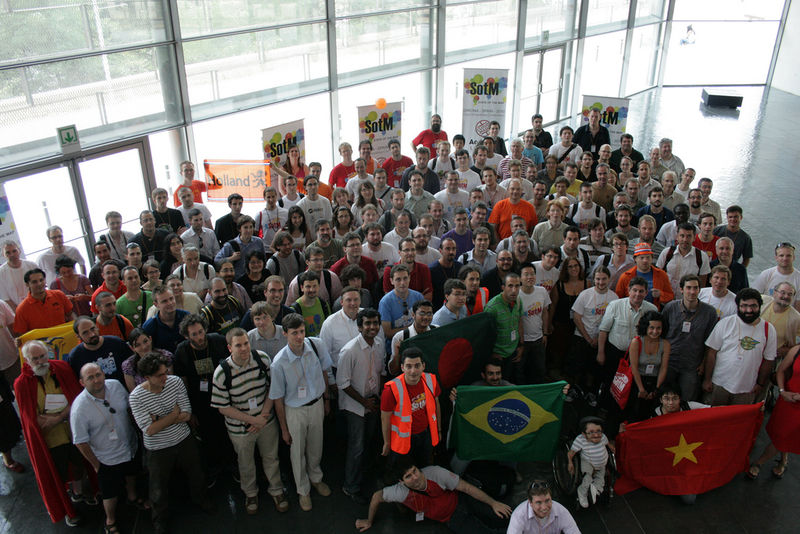
\includegraphics[width=5.5cm]{sotm.jpg}
 \end{center}

\end{frame}

\subsection{Warum OpenStreetMap}

\begin{frame}{Wir brauchen freie Karten!}
Vorhandene Geodaten
\begin{itemize}
  \item wenn gratis, dann nur für Lehre und Forschung
  \item bei kommerzieller Nutzung oft zu teuer
  \item wenn es sie denn gibt - zB Haiti
\end{itemize}

\pause
\vspace{2mm}
Karten kommerzieller Anbieter nur sehr restriktiv nutzbar
\begin{itemize}
  \item Restriktive Lizenzen - only Free as in Beer
  \item Offline-Nutzung oft nicht erlaubt - Roaming!
  \item Absichtliche Fehler, Änderungen/Richtigstellungen?
  \pause
  \item zB Bing TOS: \emph{Durch die Nutzung schließen sie einen rechtsgültigen Vertrag mit Microsoft} - Dürfen unmündige Personen (unter 18?) Bing Maps überhaupt nutzen?
  \item Kosten! Google verlangt z.B. ab 25K API-Zugriffen/Tag!
\end{itemize}

\end{frame}

{
 \usebackgroundtemplate{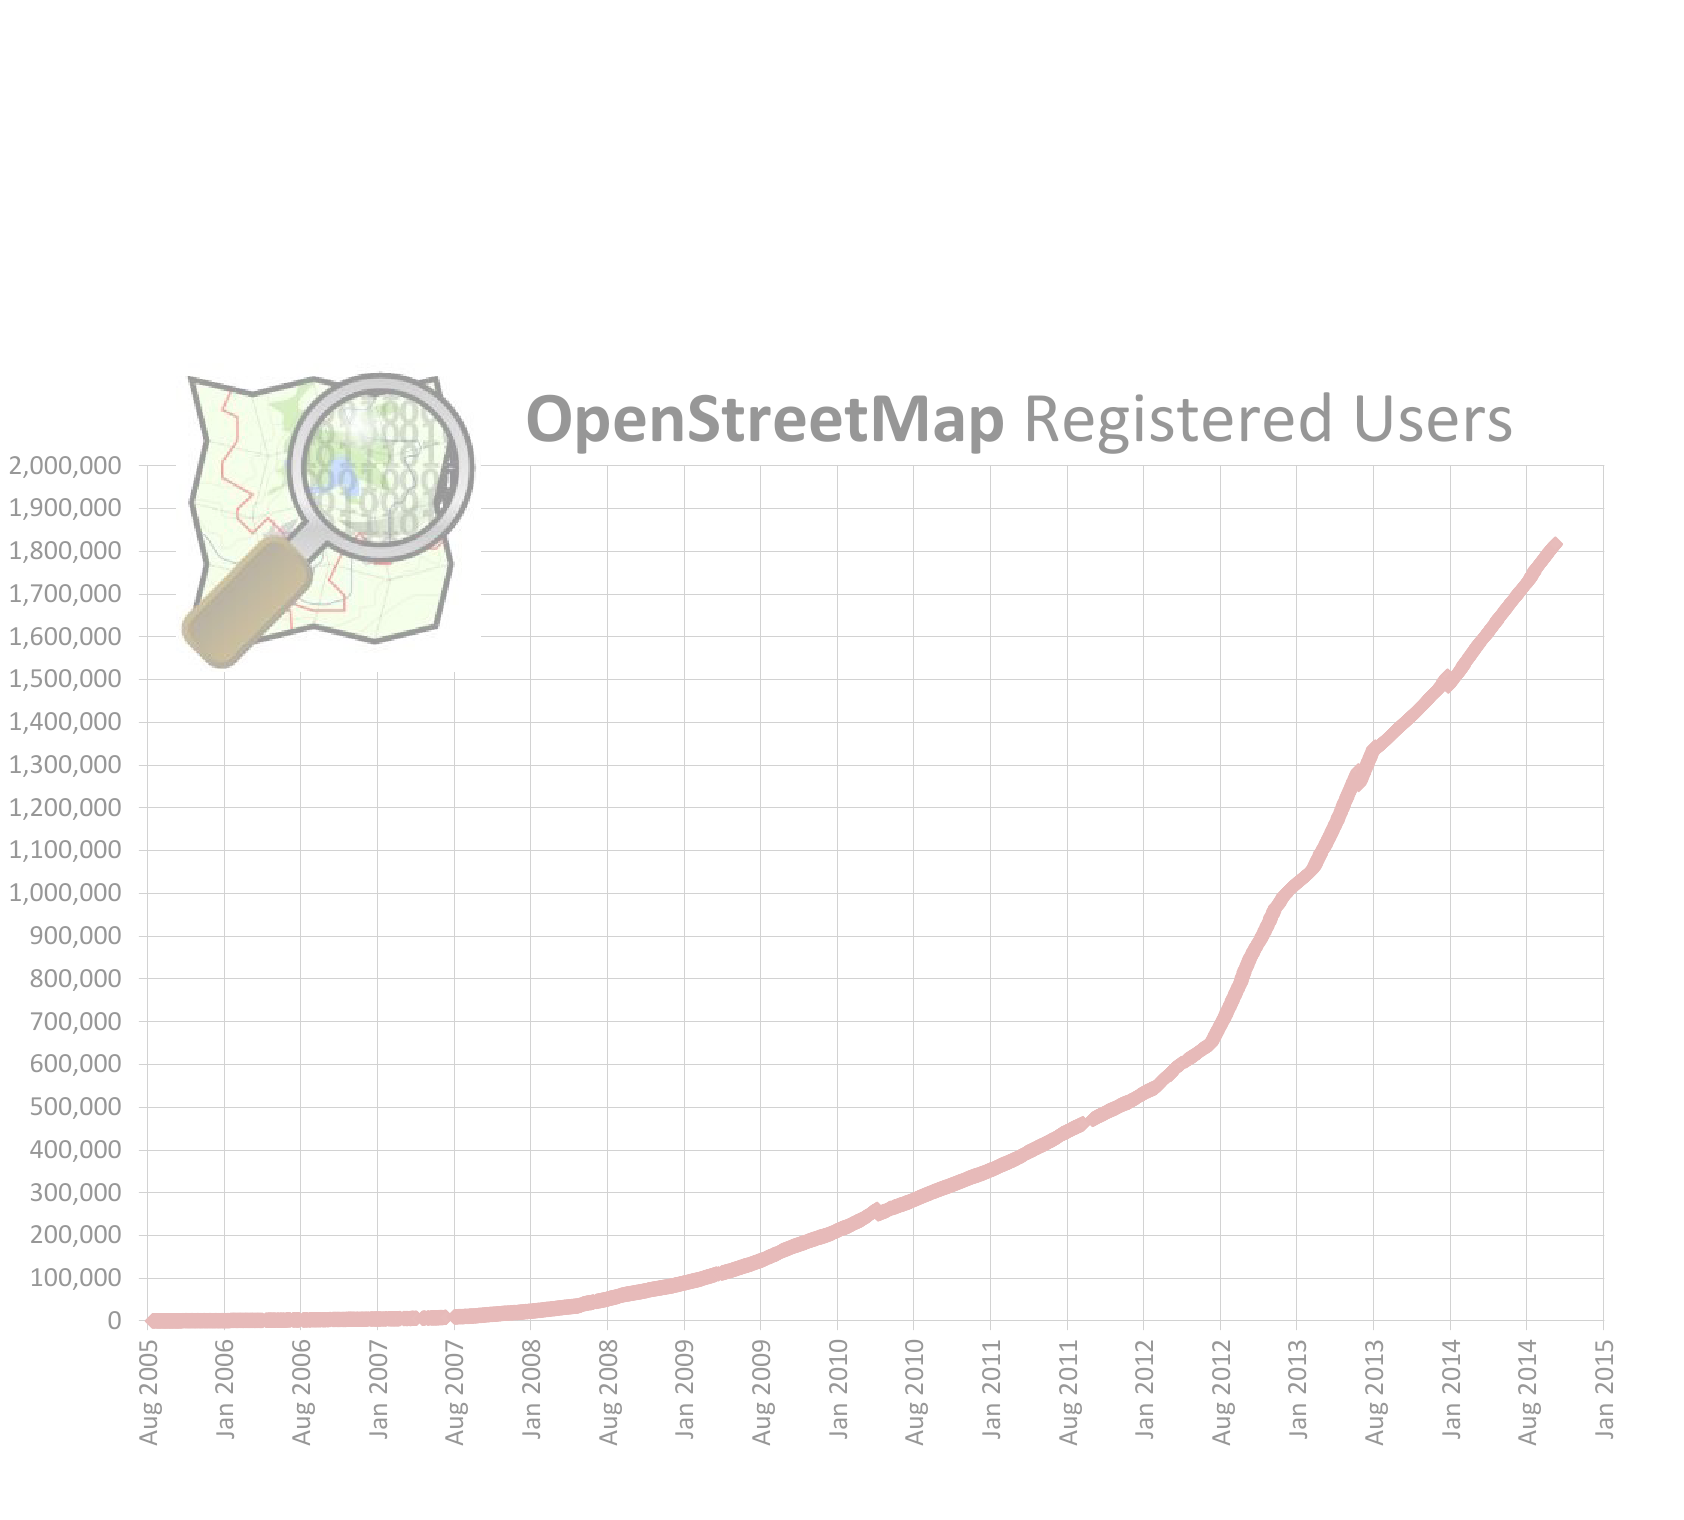
\includegraphics[height=10cm]{Osmdbstats2_users.png}} %added 20% whitespace on top of file inside png

\begin{frame}{Geschichte von OpenStreetMap}
  \vspace{0.6cm}
\begin{itemize}
  \item Start des Projekts im August 2004 durch \emph{Steve Coast}
  \item Dezember 2006 - Yahoo erlaubt abzeichnen
  \item Juli 2007 - Erste Konferenz, "`State Of The Map"'
  \item August 2007 - 10.000 Registrierte Benutzer
  \item März 2009 - 100.000 Registrierte Benutzer
  \item Januar 2010 - Haiti--Projekt
  \item November 2010 - Bing erlaubt abzeichnen
  \item Juli 2011 - Erste "`State Of The Map Europe"' in Wien
  \item Januar 2013 - 1.000.000 Registrierte Benutzer
  \item Gestern - 1.874.330 Registrierte Benutzer
\end{itemize}

\end{frame}
}


\begin{frame}{Wer steht hinter OpenStreetMap}

  \begin{itemize}
    \item OpenStreetMap Foundation (Dataserver, Rechtsvertretung)
      \pause
    \item "`Mapper"' ($\sim$25.000 aktiv), meist ohne Geo-Hintergrund
    \begin{itemize}
      \item Jährliche Konferenz - "`State of the Map"', heuer: Buenos Aires
    \end{itemize}
      \pause
    \item Universitäten:
    \begin{itemize}
      \item Bakk-, Master- und Doktorarbeiten mit OSM
      \item Server-Hosting
    \end{itemize}
      \pause
    \item Organisationen, die Daten sponsern:
    \begin{itemize}
      \item Firmen wie Yahoo/Bing, die Luftbilder zur Verfügung stellen
      \item Regierungen mit besseren Open-Data-Gesetzen als Österreich 
  % BSP TIGER, USA
  % Dänemark, Hausnummern
  % Frankreich,Tschechien: Kataster
    \end{itemize}
      \pause
    \item Firmen, die Dienste rund um OSM anbieten:
    \begin{itemize}
      \item Geofabrik (de)
      \item MapBox (us)
      \item BikeCityGuide (Graz)
    \end{itemize}
  \end{itemize}

\end{frame}

% aufteilung:
% OSMF stellt die Infrastruktur für Rohdaten zur Verfügung.
% Kommerzielle Dienste (Tileserver, spezialisierte Extraket) - Firmen
  


\section{Wie funktioniert OpenStreetMap?}

\begin{frame}{Woher kommen unsere Daten?}

  \vspace{-1.7cm}
\begin{columns}
\begin{column}[l]{5cm}
\end{column}
\begin{column}[r]{4cm}
 \begin{figure}
        \includegraphics<1>[width=4.7cm]{gpx.png}
        \includegraphics<2>[width=4.7cm]{gpx-aerial.png}
        \includegraphics<3>[width=4.7cm]{gpx-aerial-names.png}
        \includegraphics<4>[width=4.7cm]{gpx-aerial-names-pois.png}
        \includegraphics<5>[width=4.7cm]{gpx-aerial-names-pois.png}
    \end{figure}   
\end{column}
\end{columns}

  \vspace{-4cm}

\begin{itemize}
  \item Am Anfang: GPS-Tracks
\pause
  \item Luftbilder    
\pause
  \item Mapper digitalisieren die Rohdaten
  \item Jeder kann sein Wissen beitragen:
	\begin{itemize}
	  \item Straßennamen\pause, Hausnummern
	  \item Restaurants, Bars, POIs, \dots
  \end{itemize}
\end{itemize}

  \vspace{0.3cm}
 99\% Handarbeit!
  \vspace{0.3cm}


  \pause
\begin{itemize}
  \item Unterstützt durch Open Government Data
  \begin{itemize}
    \item USA, TIGER Data (2008)
    \item Dänemark, Hausnummern (laufend synchronisiert)
    \item Graz, Steiermark, Wien, Engerwitzdorf... und 20 weitere
  \end{itemize}
\end{itemize}

\end{frame}

\begin{frame}{Qualitätssicherung}
Ähnlich Wikipedia, jeder darf alles ändern!
  \begin{columns}[c]
    \begin{column}[T]{.35\textwidth}
      \vspace{1cm}
      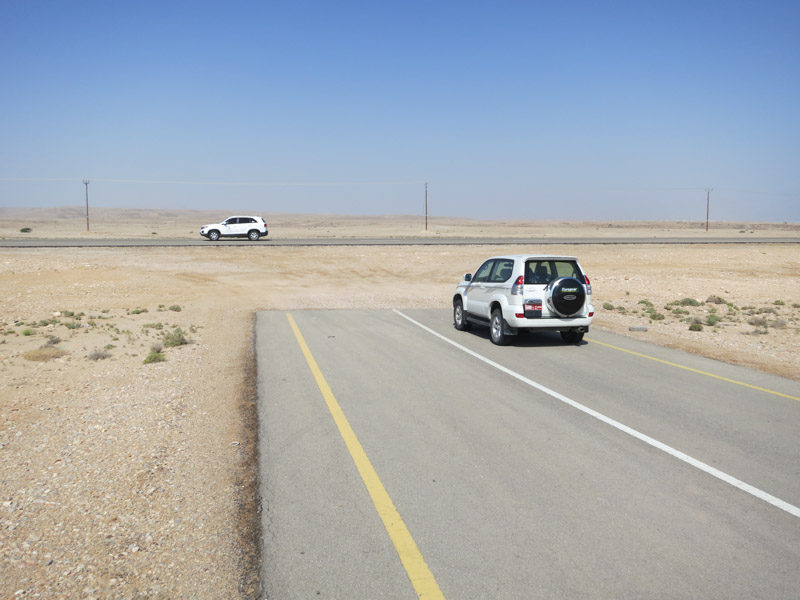
\includegraphics[width=4.5cm]{unconnected.jpg} \\
      {\TINY CC-BY \url{http://www.bodenseepeter.de}}
    \end{column}
    \pause
    \begin{column}[T]{.7\textwidth}
      \begin{itemize}
        \item Jedoch konfliktfreier als bei Wikipedia:
        \begin{itemize}
          \item Es gibt in OSM nur "`Ground Truth"'
          \item Eintrittsschwelle ist höher (keine Anonymous edits)
        \end{itemize}
        \item Erfahrene Mapper kontrollieren ihr Gebiet mittels RSS-Feed
        \pause
        \item Eingebautes Social Network: Jeder Mapper kann persönlich kontaktiert werden
        \begin{itemize}
          \item Diskussion über die Mailingliste
        \end{itemize}
        \pause
        \item Automatische Qualitätssicherungs-Tools
        \begin{itemize}
          \item \href{http://keepright.ipax.at/report\_map.php?zoom=14&lat=48.20808&lon=16.37221}{keepright.ipax.at}
        \end{itemize}
      \end{itemize}

    \end{column}
  \end{columns}

\end{frame}

\begin{frame}{Welche Daten sind in der OSM}
  Was erfassen wird erfasst? Beinahe \emph{Alles} ... mit Geobezug
\pause
  \begin{itemize}
    \item Straßen, Wege, Eisenbahnen
    \item Landnutzungen, Flüsse
    \item Städte, Gebäude, Hausnummern
    \item Grenzen
    \item Berge, Höhlen, Wasserflächen
    \item Geschäfte und POIs, Denkmäler, Bäume
    \item ÖPNV-, Rad- und Wanderrouten
    \item Interdatabase-Links zu Wikipedia und Wikidata
\end{itemize}
\end{frame}

\begin{frame}{Vorteile von OSM}

Was unterscheidet die OSM von anderen Karten

  \begin{itemize}
    \item Rohdaten frei
    \item minütlich Aktuell
    \item Multilanguage-Support
    \item vollständige Versionierung
    \item offenes Tagging-System
    \item nicht zensierbar
    \item Fehler melden oder sofort korrigieren
    \item 100 \% Freie Software
    \item Web-Karten kompatibel zu kommerziellen APIs
    \item beliebige Kartenstile
\end{itemize}
\end{frame}
 
\subsection{Anwendungen}

\hypersetup{urlcolor=cyan}

\begin{frame}{Beispielkarte: \hfill\href{http://www.OpenStreetMap.org}{OpenStreetMap.org}}

 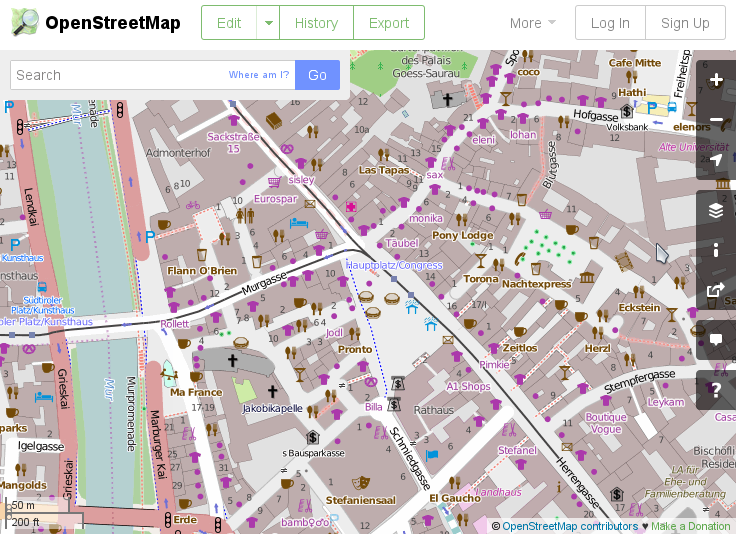
\includegraphics[width=11cm]{osmorg.png}

\end{frame}

\begin{frame}{Stamen Watercolor:\hfill\href{http://maps.stamen.com/watercolor/}{maps.stamen.com/watercolor}}
\begin{center}
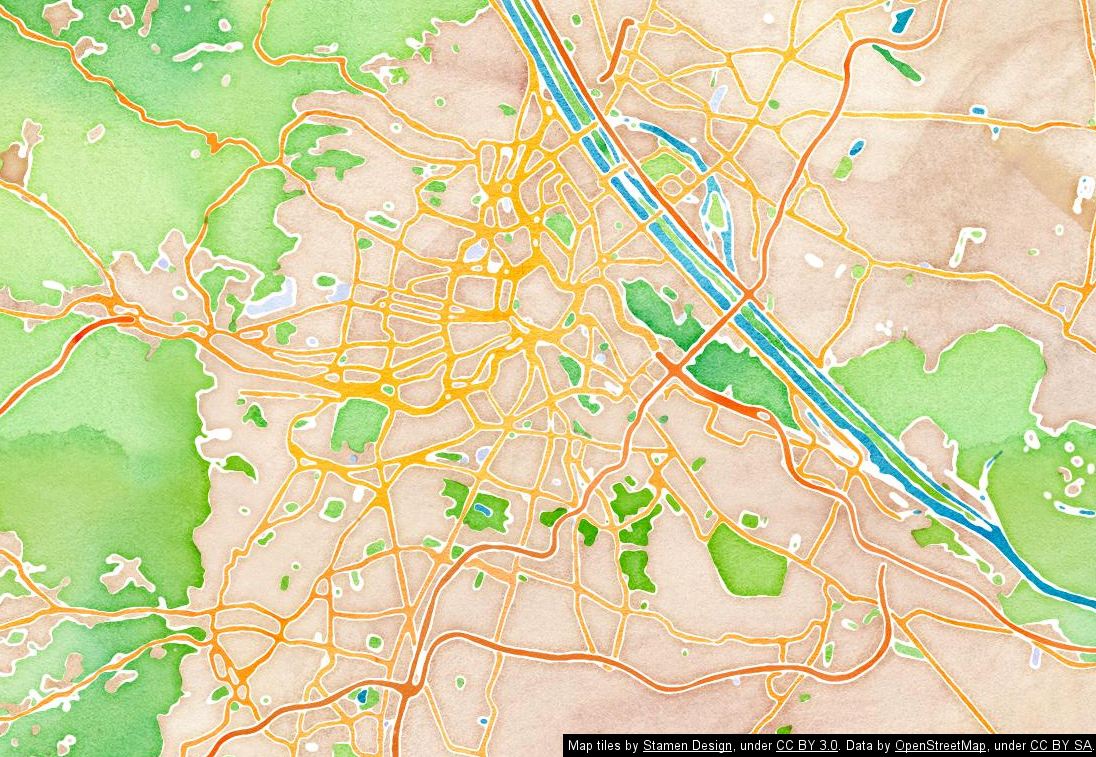
\includegraphics[height=7cm]{style-stamen.png}
\end{center}
\end{frame}

\begin{frame}{Fahrrad-Karte :\hfill\url{http://www.opencyclemap.org}}
  \vspace{-0.3cm}
\begin{center}
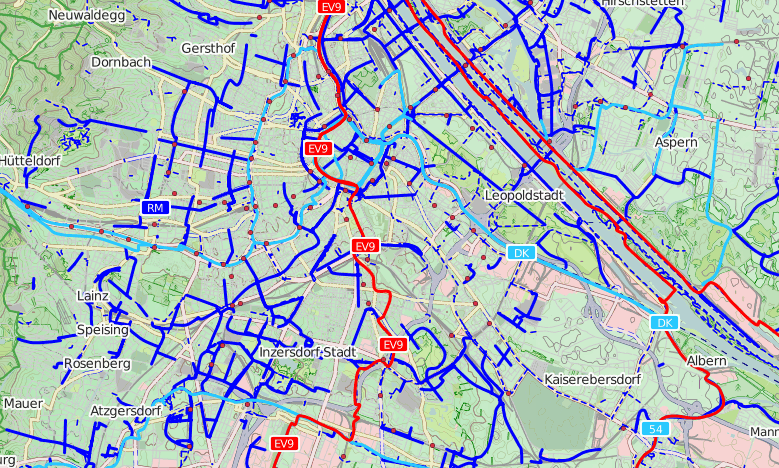
\includegraphics[height=6.7cm]{style-cycle.png}
\end{center}
\end{frame}

\begin{frame}{See-Karte :\hfill\url{http://www.openseamap.org}}
\begin{center}
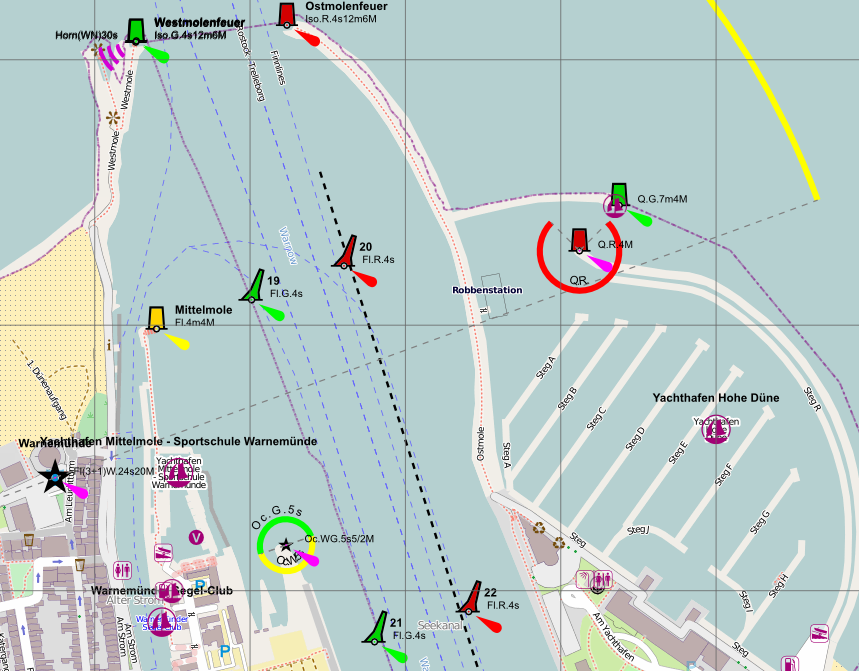
\includegraphics[height=7cm]{style-seamap.png}
\end{center}
\end{frame}

\begin{frame}{Nichtraucher-Karte :\hfill\url{http://www.opengastromap.de}}
\begin{center}
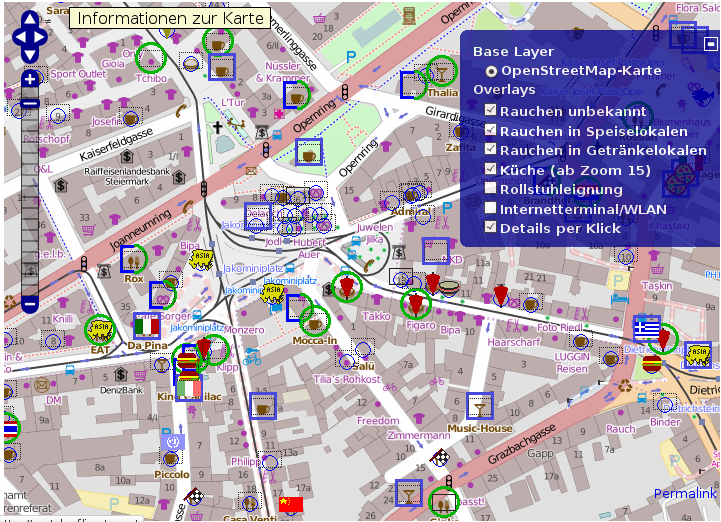
\includegraphics[height=7cm]{smoking.png}
\end{center}
\end{frame}

\hypersetup{urlcolor=blue}


\begin{frame}{Was ist noch mit OSM möglich}

  \vspace{-1.9cm}
\begin{columns}
\begin{column}[l]{5cm}

\end{column}
\begin{column}[r]{4cm}
 \begin{figure}
        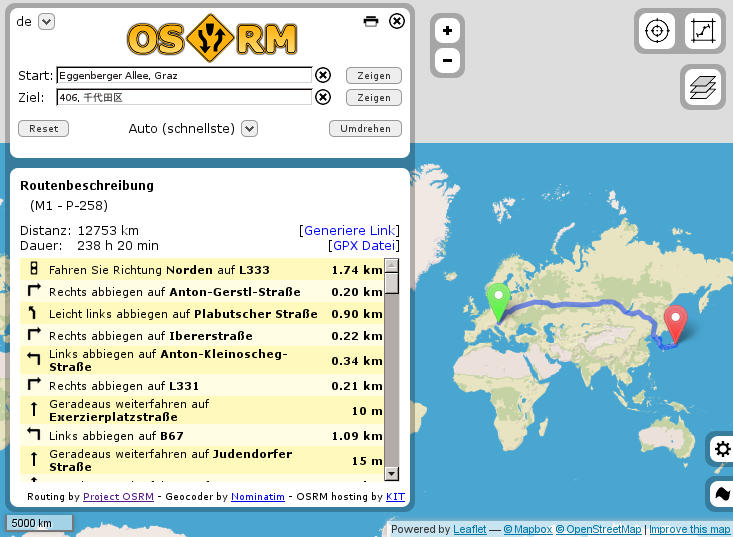
\includegraphics[width=5.2cm]{osrm.png}
    \end{figure}   
\end{column}
\end{columns}

  \vspace{-4cm}

Weitere Anwendungsgebiete:
\begin{itemize}
    \item Routing:
    \begin{itemize}
        \item zB: Fahrrad, Rollstuhl
        \item über 150 Apps, und für Garmin
    \end{itemize}
    \item Analysen, z.B.:
    \begin{itemize}
        \item Straßennetz, Erreichbarkeit
        \item Administrative Flächen
    \end{itemize}
    \item Geocoding, Reverse-Geocoding
    \item Einbinden in die Eigene Website, Verlinkungen
    \item Lokalisierte Karten
    
\end{itemize}

\end{frame}


\hypersetup{urlcolor=cyan}

\begin{frame}{Lokalisierte Karten:}
\begin{center}
\vspace{-1cm}
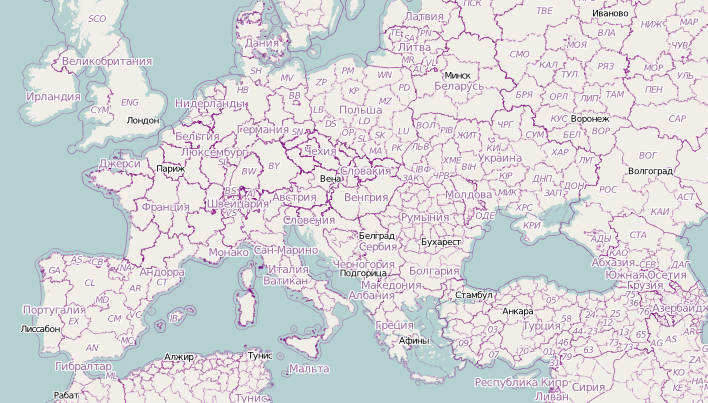
\includegraphics[height=6.5cm]{style-russ.png}
\end{center}
\end{frame}

\hypersetup{urlcolor=blue}


% was kann ich nun mit diesem Schatz an Rohdaten machen
% • -Bunte- verschiedenste Karten
%   · Fahrrad -OK
%   · Rauchfrei -OK
%   · ÖPNV -NOK
%   · Seamap -OK
% • Routing
%  · Online, Offline, Fahrrad, Rollstuhl
% • Analysen (zB ÖPNV-Erreichbarkeit)
% • Einbinden in die Eigene Website
% • Geocoding + Reverse



% folien: OGD

\section{Open Government Data}

\begin{frame}{Open Government Data}

Unterschiedliche Einstellungen:
\begin{itemize}
    \item USA: was ein Bundesbeamter macht: Public Domain :-)
    \begin{itemize}
        \item  \href{http://data.gov}{data.gov}: 250.000 datasets
    \end{itemize}
    \item AT: was ein Beamter macht: Amtsgeheimnis :-/
    \begin{itemize}
        \item \href{data.gv.at}{data.gv.at}: 1.508 Datensätze
    \end{itemize}
\end{itemize}

\pause

Problem in AT: 
\begin{itemize}
    \item Zuständige Behörde muss jeden Datensatz einzeln freigeben
    \item Ablauf verkehrt: Eigentlich sollt's automatisch auf data.gv.at
\end{itemize}
\pause
Gutes Beispiel: Land Vorarlberg: 
\begin{itemize}
    \item Ihr Arbeitsserver: scp-server vogis@vogis.cnv.at 
    \item Mit SSH hinverbinden, mit SCP herunterladen 
    \item 'Nehmt was ihr braucht'
    \begin{itemize}
        \item Grenzen (Länder, Bezirke Österreichweit)
        \item Höhenmodell
        \item Verkehr, Wasser
        \item Naturschutzgebiete, Raumplanung
    \end{itemize}
\end{itemize}

\end{frame}


% TransforMap

%\begin{frame}{}
%\end{frame}



%\section{OpenStreetMap Nutzen}


\begin{frame}{OpenStreetMap - jetzt auch in 3D! }
    auf \href{http://maps.osm2world.org/?zoom=17&lat=47.06156&lon=15.46983&layers=BF0FTFFF}{maps.osm2world.org} oder in der DAVE, Inffeldg. 25 (CGV)

  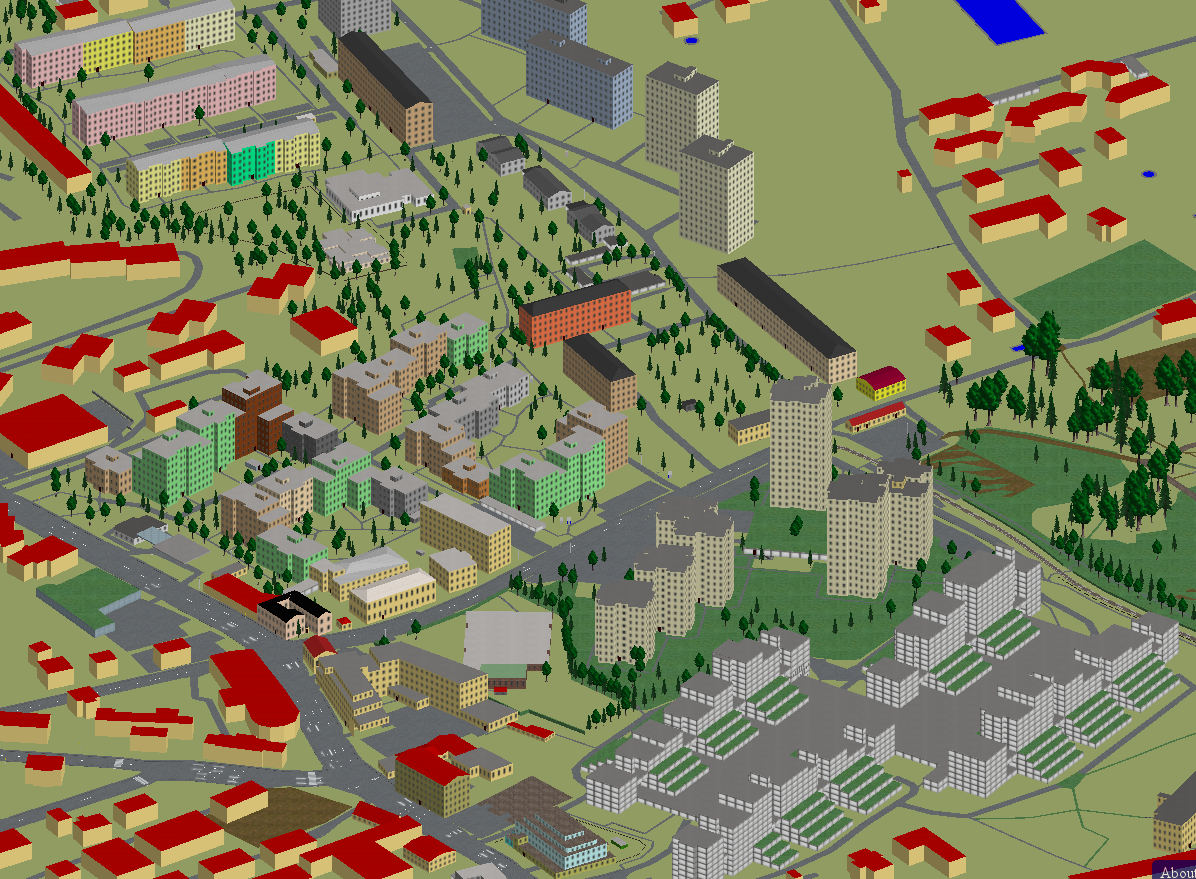
\includegraphics[width=0.9\textwidth]{3d.png}


\end{frame}

\section{Ende}

\begin{frame}{Hilfe}
Fragen? 
\begin{itemize}
  \item OSM-Wiki: \href{http://wiki.openstreetmap.org}{wiki.openstreetmap.org}
  \begin{itemize} 
    \item Mitmachen? \href{http://learnosm.org/}{learnosm.org}
  \end{itemize}
  \item Fragen stellen? \\ $\Rightarrow$ Mailingliste \href{http://lists.openstreetmap.org/listinfo/talk-at}{talk-at}
\vspace{1cm}
  \item Grazer \href{https://wiki.openstreetmap.org/wiki/Graz/Stammtisch}{Stammtisch}
  \begin{itemize}
      \item jeden 2. Montag im Monat 
      \item Brot $\&$ Spiele
  \end{itemize}

\end{itemize}

 \vspace*{-2.0cm}
\hfill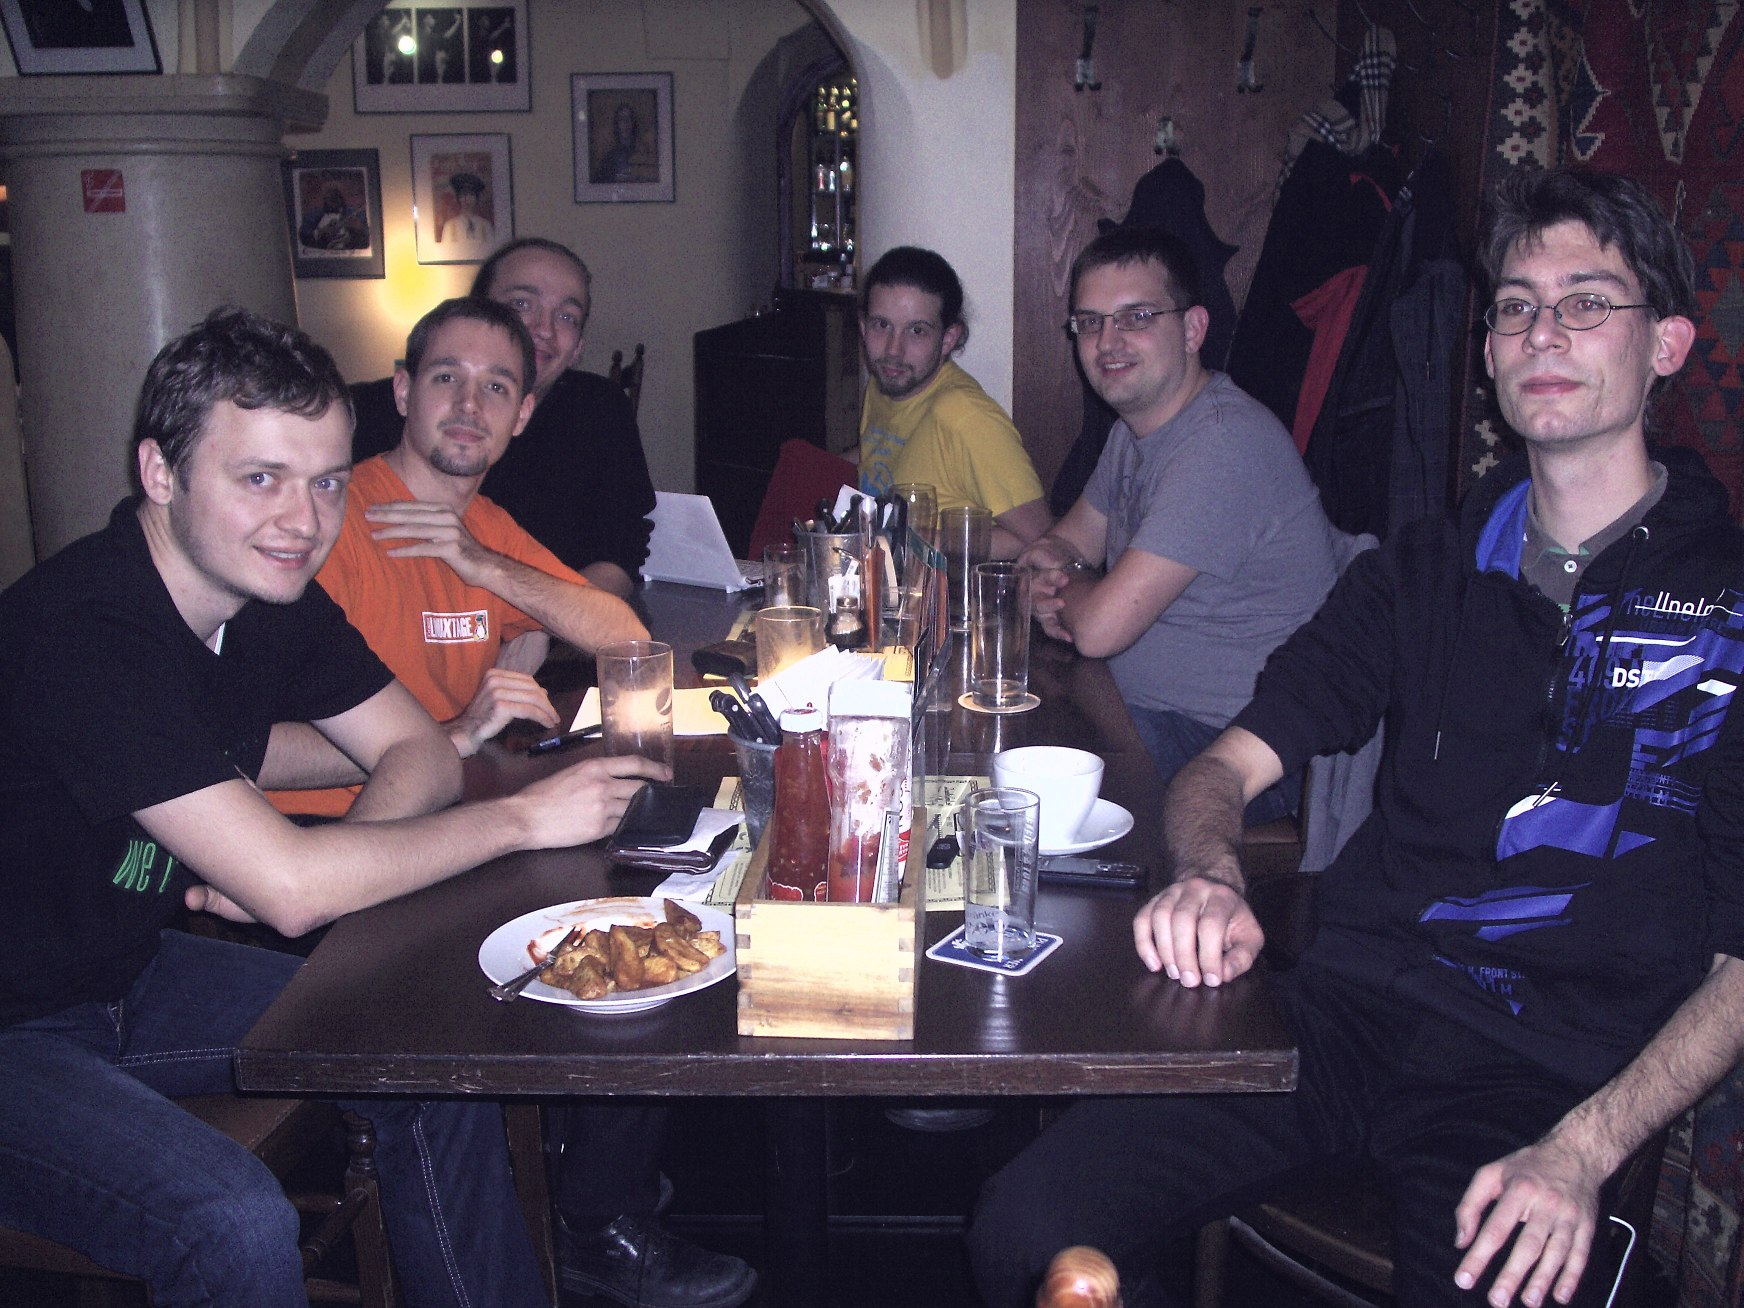
\includegraphics[width=5cm]{Osm_graz_members_2011.jpeg}

\end{frame}

\begin{frame}{Vielen Dank für die Aufmerksamkeit!}

  Folien zum Austria-Forum Jour-Fix, 26.11.2014, Graz
\vspace{1cm}

Erstellt mittels \LaTeX Beamer, Quelltext: \href{https://github.com/species/vortrag-osm-austriaforum}{Github}.
\vspace{1cm}

\href{mailto:michael.maier@student.tugraz.at}{Michael Maier}

Twitter: \href{https://twitter.com/osmgraz}{@osmgraz}
\vspace{1cm}

Folien unter: 
\includegraphics[width=1cm]{cc-by-sa.pdf}. 

\vspace{0.2cm}
Alle Daten ODbL, OpenStreetMap Contributors.

\end{frame}


\end{document}
